\documentclass{standalone}
\usepackage{tikz}
\begin{document}
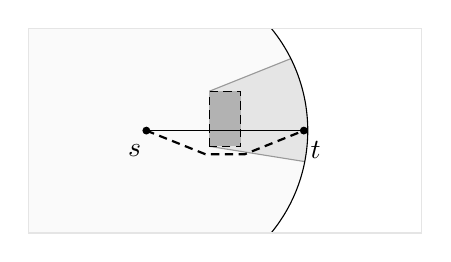
\begin{tikzpicture}

%\begin{scope}
%   \clip (0.0,-1.3) rectangle (5.0,1.3);
%   \fill[black!5] (1.5,0.0) circle (2.05);
%   \draw (1.5,0.0) circle (2.05);
%\end{scope}

\begin{scope}
   \clip (0.0,-1.3) rectangle (5.0,1.3);
   
   % initial search
   \fill[black!2] (1.5,0.0) circle (2.05);
   
   % reduced step-2 subset
   \begin{scope}
      \clip (1.5,0.0) circle (2.05);
      \fill[black!10] (2.3,0.5) -- (3.55,1.0) -- (3.55,-0.4) -- (2.3,-0.2) -- cycle;
      \draw[black!40] (2.3,0.5) -- (3.55,1.0);
      \draw[black!40] (3.55,-0.4) -- (2.3,-0.2);
   \end{scope}
   
   % initial search boundary
   \draw (1.5,0.0) circle (2.05);
\end{scope}

% new obstacle
\draw[fill=black!30,densely dashed] (2.3,-0.2) rectangle (2.7,0.5);

\fill[black] (1.5,0.0) circle (0.05);
\node at (1.35,-0.25) {$s$};
\fill[black] (3.5,0.0) circle (0.05);
\node at (3.65,-0.25) {$t$};

% old path
\draw (1.5,0.0) -- (3.5,0.0);

% new path
\draw[thick,densely dashed] (1.5,0.0) -- (2.25,-0.3) -- (2.75,-0.3) -- (3.5,0.0);

% border
\draw[black!10] (0.0,-1.3) rectangle (5.0,1.3);

\end{tikzpicture}%
\end{document}
